The performances of the inverse subspace iteration for 50 and 500 eigenvalues:

\begin{figure}[H]
  \centering
  \begin{subfigure}[b]{0.5\textwidth}
   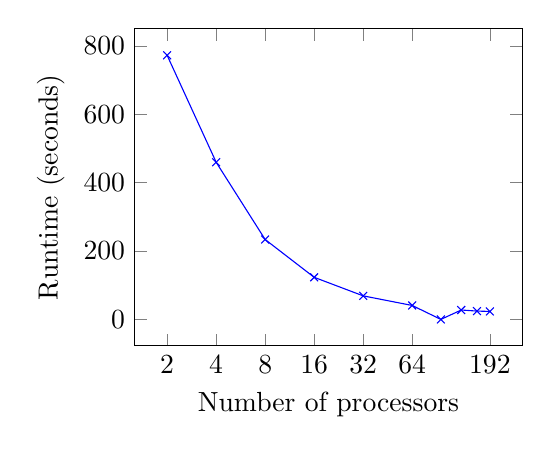
\begin{tikzpicture}
 \begin{axis}[
  width=6.5cm,
  xlabel=Number of processors,
  xtick={2, 4, 8, 16, 32, 64, 192},
  xmode=log,
  log ticks with fixed point,
  ylabel=Runtime (seconds)]
   \addplot[color=blue, mark=x] coordinates {
    (2, 772.2112808)
    (4, 459.5902418)
    (8, 233.5733138)
    (16, 123.080028)
    (32, 68.868284)
    (64, 40.7892172)
    (96, 0)
    (128, 27.5095412)
    (160, 24.3766952)
    (192, 23.3256756)
   };
 \end{axis}
\end{tikzpicture}

   \caption{50 eigenvalues.}
  \end{subfigure}
  \begin{subfigure}[b]{0.45\textwidth}
   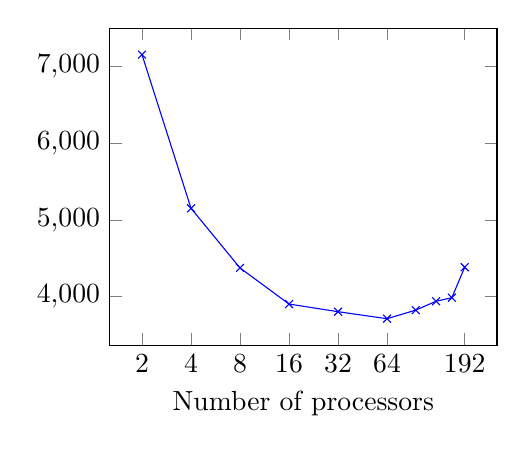
\begin{tikzpicture}
 \begin{axis}[
  width=6.5cm,
  xlabel=Number of processors,
  xtick={2, 4, 8, 16, 32, 64, 192},
  xmode=log,
  log ticks with fixed point]
  %ylabel=Runtime (seconds)]
   \addplot[color=blue, mark=x] coordinates {
    (2, 7149.885403)
    (4, 5149.912356)
    (8, 4373.481026)
    (16, 3903.60577)
    (32, 3803.859549)
    (64, 3712.591258)
    (96, 3824.621957)
    (128, 3939.533307)
    (160, 3986.572888)
    (192, 4383.063958)
   };
 \end{axis}
\end{tikzpicture}

   \caption{500 eigenvalues.}
  \end{subfigure}
  \caption{Runtime of the inverse subspace iteration part of the algorithm.}
\end{figure}

When increasing a low number of processors, we see a sharp improvement of the performances in both cases.
But the runtime stagnates quickly when the number of processors grows and we even observe a raise of the runtime.
The algorithm reaches its parallelisation limit and the communication overhead takes over.

We know from the runtime performances that the inverse iteration part of the algorithm is not scaling correctly.
For any amount of computed eigenvalues, when we increase the number of processes, the proportion of time spent computing the eigenvalues increases.
For 500 eigenvalues and 128 processors, we spend more than 99\% of the time computing the eigenvalues.
This confirms that the algorithm does not quite scale yet.

We now have a look at the internal steps of the inverse power method to see where lies the problem.
The algorithm consists of iteratively solving \(m\) linear systems, orthonormalising the vectors and computing the residual norm.
Here is the proportion of each step of the inverse subspace interation for the computation of 50 and 500 eigenvalues:

\begin{figure}[H]
  \centering
  \begin{tikzpicture}
 \begin{groupplot}[
  group style={
   group size=2 by 1,
   xlabels at=edge bottom,
   ylabels at=edge left,
   },
  ybar stacked,
  ymin=0,
  ymax=100,
  height=7cm,
  width=0.5\textwidth,
  xlabel=Number of processors,
  ylabel={Percentage (\%)},
  symbolic x coords={2, 4, 8, 16, 32, 64, 96, 128, 160, 192},
  legend style={
   at={(0, -0.25)},
   anchor=north}
  ]
  \nextgroupplot[title={50 eigenvalues.}]
  \addplot[ybar, fill=blue] plot coordinates {
   (2, 8.14)
   (4, 6.16)
   (8, 5.98)
   (16, 9.09)
   (32, 13.50)
   (64, 18.56)
   (96, 22.42)
   (128, 25.35)
   (160, 27.53)
   (192, 29.06)};
  \addplot[ybar, fill=red] plot coordinates {
   (2, 0.46)
   (4, 0.96)
   (8, 2.01)
   (16, 3.90)
   (32, 7.31)
   (64, 13.29)
   (96, 17.61)
   (128, 20.94)
   (160, 23.90)
   (192, 26.27)};
  \addplot[ybar, fill=yellow] plot coordinates {
   (2, 85.67)
   (4, 86.96)
   (8, 86.16)
   (16, 81.40)
   (32, 73.91)
   (64, 63.23)
   (96, 55.21)
   (128, 49.07)
   (160, 43.95)
   (192, 40.00)};
  \addplot[ybar, fill=green] plot coordinates {
   (2, 5.74)
   (4, 5.92)
   (8, 5.84)
   (16, 5.61)
   (32, 5.28)
   (64, 4.91)
   (96, 4.76)
   (128, 4.64)
   (160, 4.62)
   (192, 4.68)};

  \nextgroupplot[title={500 eigenvalues.}]
  \addplot[ybar, fill=blue] plot coordinates {
   (2, 23.76)
   (4, 15.29)
   (8, 11.43)
   (16, 12.30)
   (32, 11.68)
   (64, 9.84)
   (96, 9.47)
   (128, 9.75)
   (160, 9.57)
   (192, 9.39)};
  \addplot[ybar, fill=red] plot coordinates {
   (2, 46.02)
   (4, 63.07)
   (8, 75.14)
   (16, 79.65)
   (32, 83.37)
   (64, 86.81)
   (96, 87.72)
   (128, 87.77)
   (160, 88.07)
   (192, 88.50)};
  \addplot[ybar, fill=yellow] plot coordinates {
   (2, 28.78)
   (4, 20.15)
   (8, 11.97)
   (16, 6.60)
   (32, 3.49)
   (64, 1.84)
   (96, 1.29)
   (128, 0.98)
   (160, 0.80)
   (192, 0.64)};
  \addplot[ybar, fill=green] plot coordinates {
   (2, 1.44)
   (4, 1.48)
   (8, 1.46)
   (16, 1.46)
   (32, 1.46)
   (64, 1.51)
   (96, 1.53)
   (128, 1.50)
   (160, 1.56)
   (192, 1.47)};
  \legend{
   Solving the system of linear equations,
   Gram-Schmidt orthogonalisation,
   Residual norm computation,
   Rest overhead}
 \end{groupplot}
\end{tikzpicture}

  \caption{Proportion of each step in the inverse subspace iteration.}
\end{figure}

We observe that the Gram-Schmidt orthogonalisation is the limiting factor and is the most time-consuming step of the inverse iteration as the number of processors grows.
It is a well-known problem that the simple Gram-Schmidt process is actually difficult to parallelise efficiently.
Small optimisations for a parallel Gram-Schmidt orthogonalisation exist \cite{katagiri_parallel_gram_schmidt_2003} but they do not properly solve the problem.

This issue will be difficult to overcome completely.
But fundamentally, the orthogonalisation is used to stabilise the algorithm.
To accelerate our algorithm further, we try to orthogonalise the vectors \(X_k\) every second iteration instead of every iteration.
We present below the resulting performances:

\begin{figure}[H]
  \centering
  \begin{subfigure}[b]{0.5\textwidth}
   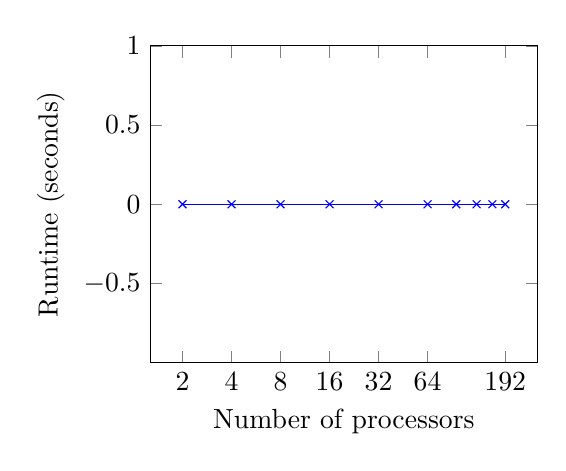
\begin{tikzpicture}
 \begin{axis}[
  width=6.5cm,
  xlabel=Number of processors,
  xtick={2, 4, 8, 16, 32, 64, 192},
  xmode=log,
  log ticks with fixed point,
  ylabel=Runtime (seconds)]
   \addplot[color=blue, mark=x] coordinates {
    (2, 0)
    (4, 0)
    (8, 0)
    (16, 0)
    (32, 0)
    (64, 0)
    (96, 0)
    (128, 0)
    (160, 0)
    (192, 0)
   };
 \end{axis}
\end{tikzpicture}

   \caption{50 eigenvalues.}
  \end{subfigure}
  \begin{subfigure}[b]{0.45\textwidth}
   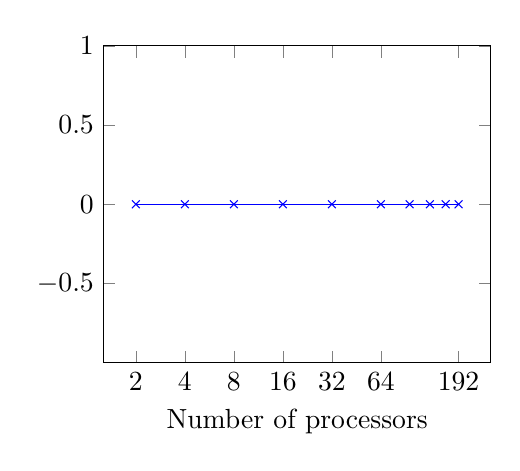
\begin{tikzpicture}
 \begin{axis}[
  width=6.5cm,
  xlabel=Number of processors,
  xtick={2, 4, 8, 16, 32, 64, 192},
  xmode=log,
  log ticks with fixed point]
  %ylabel=Runtime (seconds)]
   \addplot[color=blue, mark=x] coordinates {
    (2, 0)
    (4, 0)
    (8, 0)
    (16, 0)
    (32, 0)
    (64, 0)
    (96, 0)
    (128, 0)
    (160, 0)
    (192, 0)
   };
 \end{axis}
\end{tikzpicture}

   \caption{500 eigenvalues.}
  \end{subfigure}
  \caption{Runtime of the inverse subspace iteration part of the algorithm.}
\end{figure}

The performances for 50 eigenvalues are similar, or even a bit worse, to the ones without skipping the Gram-Schmidt orthogonalisation.
We saw that only a small proportion of time is spent doing the orthogonalisation, so the impact is not significant.

However, for computing 500 eigenvalues, the runtime with skipping the orthogonalisation every other iteration is much lower. 
Naturally, most time is spent doing the Gram-Schmidt process, which considerably speeds up the execution.
The algorithm requires more outer iterations to converge, but we nearly observe a factor 2 speed up.
The communication overhead of the method remains a problem when the number of processors is large.
